\chapterWithSubtitle{Even More Dynamic Programming, Graphs, and Basic Search}{March 18, 2021}

\section{Maximum Weight Independent Set in Trees}

\subsection{Independent Set in a Graph}
\begin{itemize}
    \item \textbf{Independent Set}: A subset of nodes $S \subseteq V$ such that there are no edges between nodes in $S$ for graph $G = (V, E)$. If $u, v \in S$, then $(u, v) \notin E$.
    \item A graph may have multiple independent sets.
\end{itemize}

\subsection{Maximum Weight Independent Set Problem}
\begin{itemize}
    \item \textit{Input}: Graph $G = (V, E)$ and weights $w(v) \geq 0$ for each $v \in V$.
    \item \textit{Goal}: Find the maximum weight independent set in $G$.
    \item We can solve it with backtracking by converting it into a sequence of decision problems:
    \begin{itemize}
        \item Number the vertices as $v_1, v_2, ..., v_3$.
        \item Decision problem: to include $v_n$ or not.
        \item Try all possibilities and let the recursion fairy take care of the remaining decisions.
        \item Find recursively optimum solutions without $v_n$ (recurse on $G - v_n$) and with $v_n$ (recurse on $G - v_n - N(v_n)$ and include $v_n$).
        \item If graph $G$ is arbitrary, there is no good ordering that results in a small number of sub-problems.
    \end{itemize}
    \item Finding the largest independent set in an arbitrary graph is extremely hard. It is the canonical NP-hard problem.
    \item In some special classes of graphs, we can find the largest independent sets quickly.
    \item For a tree graph with $n$ vertices, we can computer the maximum weight independent set in $O(n)$ time.
    \begin{itemize}
        \item \textit{Input}: Tree $T = (V, E)$ and weights $w(v) \geq 0$ for each $v \in V$.
        \item \textit{Goal}: Find the maximum weight independent set in $T$.
        \item We can use the backtracking solution described above, however a tree is special as there is a good ordering.
        \item $T(u)$: a subtree of $T$ hanging at node $u$.
        \item $OPT(u)$: the max weighted independent set value in $T(u)$.
        \begin{equation}
            OPT(u) = \max \left\{
                \begin{tabular}{c}
                    $\sum_{\text{$v$ child of $u$}} OPT(v)$ \\
                    $w(u) + \sum_{\text{$v$ grandchild of $u$}} OPT(v)$
                \end{tabular}
            \right\}
        \end{equation}
        \item There are $O(n)$ sub-problems.
        \item The base case is reaching leaf of the tree.
        \item The recurrence can be memoized using a tree, so it is easy to look up children and grandchildren.
        \item Compute $OPT(u)$ bottom up as it needs to have the computed values of all children and grandchildren of $u$. This can be done in Post-Order traversal of the tree.
        \item[] \lstinputlisting{lecture15/code/mis-tree.sudo}
        \item Space: $O(n)$, to store the value of each node of $T$.
        \item Running Time:
        \begin{itemize}
            \item Naive bound: $O(n^2)$ since each $M[v_i]$ evaluation may take $O(n)$ time and there are $n$ evaluations.
            \item Better bound: $O(n)$ because a value $M[v_j]$ is accessed only by its parent and grandparent.
        \end{itemize}
    \end{itemize}
\end{itemize}

\section{Graph Basics}

\subsection{Why Graphs?}
\begin{itemize}
    \item Many important and useful optimization problems are graph problems.
    \item Two levels of resolution:
    \begin{itemize}
        \item Classic graph algorithms
        \item Modeling a problem as a graph problem and solving it using the classic algorithms
    \end{itemize}
\end{itemize}

\subsection{Graphs}
\begin{itemize}
    \item \textbf{Graph} (undirected simple) $G = (V, E)$: a two-tuple:
    \begin{itemize}
        \item $V$ is a set of vertices (also referred to as nodes)
        \item $E$ is a set of edges where each edge $e \in E$ is a set of the form $\{ u, v \}$ with $u, v \in V$ and $u \neq v$.
    \end{itemize}
    \item Graphs are just a way of encoding pairwise relationships.
    \item \textit{Notation}: An edge in an undirected graph is an unordered pair of nodes and hence it is a set. Conventially, we use $(u, v)$ for $\{ u, v \}$ when it is clear from the context that the graph is undirected.
    \item $u$ and $v$ are the end points fo an edge $\{ u, v \}$.
\end{itemize}

\subsection{Graph Representations}
\begin{itemize}
    \item Adjacency Matrix
    \begin{itemize}
        \item Represent $G = (V, E)$ with $n$ vertices and $m$ edges using a $n \times n$ adjacency matrix $A$.
        \item $A[i, j] = A[j, i] = 1$ if $\{ i , j \} \in E$, and $A[i, j] = A[j, i] = 0$ if $\{ i, j \} \notin E$.
        \item Advantage: can check if $\{ i, j \} \in E$ in $O(1)$ time.
        \item Disadvantage: requires $\Omega(n^2)$ space even when $m \ll n^2$.
    \end{itemize}
    \item Adjacency Lists
    \begin{itemize}
        \item Represent $G = (V, E)$ with $n$ vertices and $m$ edges using adjacency lists.
        \item For each $u \in V$, $Adj(u) = \{ v \mid \{ u, v \} \in E \}$, that is neighbors of $u$. Sometimes, $Adj(u)$ is the list of edges incident to $u$.
        \item Advantage: space is $O(m + n)$.
        \item Disadvantage: cannot "easily" determine in $O(1)$ time whether $\{ i, j \} \in E$.
        \begin{itemize}
            \item By sorting each list, $O(\log n)$ time can be achieved.
            \item By hashing "appropriately", $O(1)$ time can be achieved.
        \end{itemize}
    \end{itemize}
\end{itemize}

\subsection{A Concrete Representation of Adjacency Lists}
\begin{itemize}
    \item Assume vertices are numbered arbitrarily as $\{ 1, 2, ..., n \}$.
    \item Edges are numbered arbitrarily as $\{ 1, 2, ..., m \}$.
    \item Edges are stored in an array/list of size $m$. $E[j]$ is the $j$th edge with info on end points which are integers in the range of $1$ to $n$.
    \item An array $Adj$ of size $n$ for adjacency lists. $Adj[i]$ points to the adjacency list of vertex $i$. $Adj[i]$ is a list of edge indices in range $1$ to $m$.
    \item[] 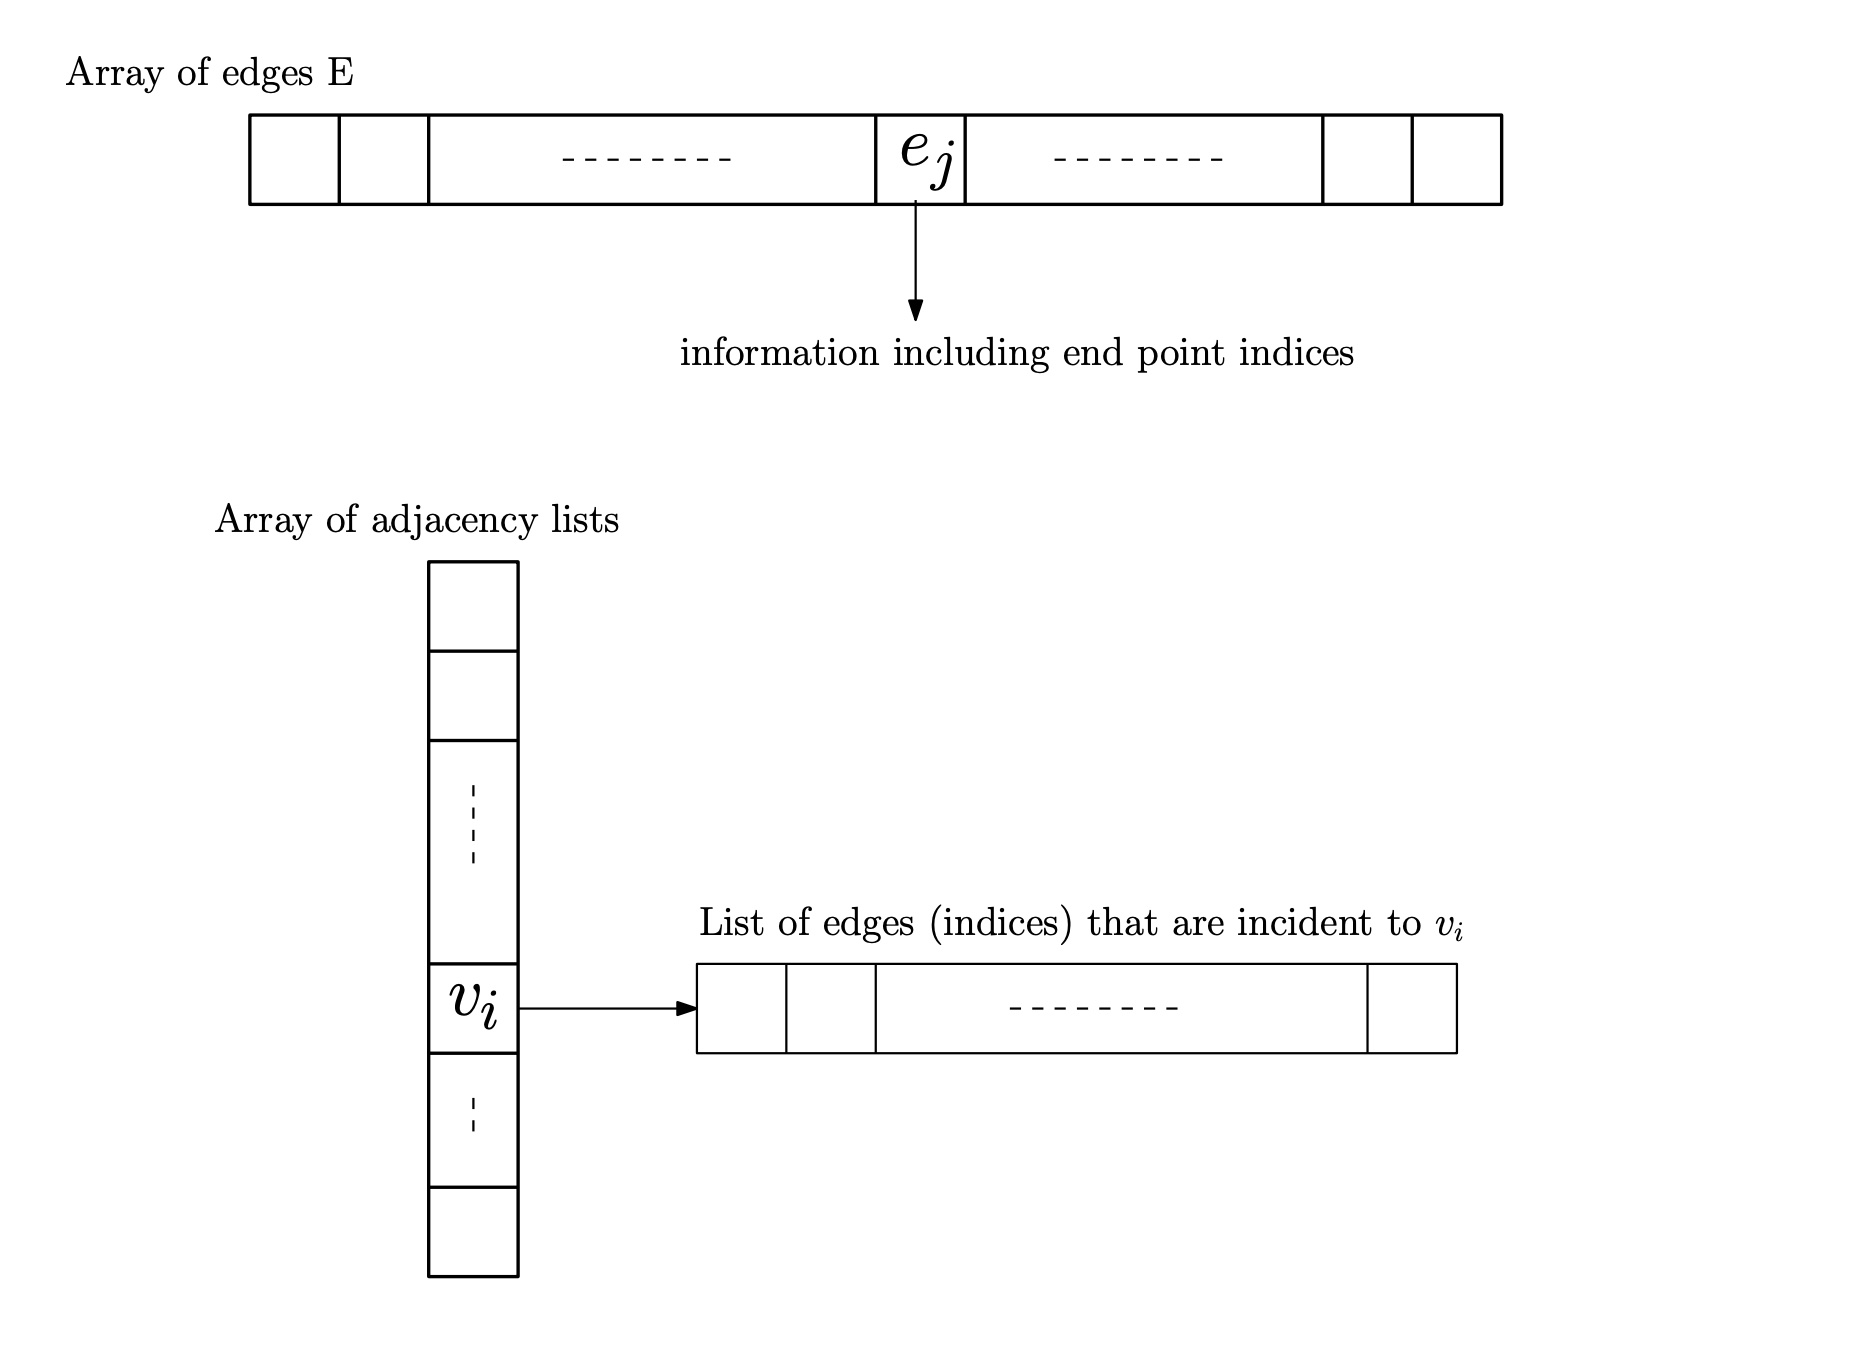
\includegraphics[width=0.8\textwidth]{lecture15/images/adjacency-list-representation.jpg}
\end{itemize}

\subsection{Connectivity on Undirected Graphs}
\begin{itemize}
    \item \textbf{Path}: a sequence of distinct vertices $v_1, v_2, ..., v_k$ such that $\{ v_i, v_{i + 1} \} \in E$ for $1 \leq i \leq k - 1$. The length of the path is $k - 1$ (the number of edges in the path) and the path is from $v_1$ to $v_k$. A single vertex $u$ is a path of length $0$.
    \item \textbf{Cycle}: a sequence of distinct vertices $v_1, v_2, ..., v_k$ such that $\{ v_i, v_{i + 1} \in E$ for $1 \leq i \leq k - 1$ and $\{ v_1, v_k \} \in E$. A single vertex is not a cycle according to this definition.
    \item \textbf{Connected}: a vertex $u$ is connected to $v$ if there is a path from $u$ to $v$.
    \item \textbf{Connected Component}: the connected component of $u$, $con(u)$, is the set of all vertices connected to $u$.
    \item In undirected graphs, connectivity is a reflexive, symmetric, and transitive relation. Connected components are the equivalence classes.
    \item A graph is connected if only connected component exists.
    \item Connectivity problems on undirected graphs can be accomplished in $O(m + n)$ time using a basic search procedure.
    \begin{itemize}
        \item Given graph $G$ and nodes $u$ and $v$, is $u$ connected to $v$?
        \item Given $G$ and node $u$, find all nodes that are connected to $u$.
        \item Find all connected components of $G$.
    \end{itemize}
\end{itemize}

\subsection{Basic Graph Search in Undirected Graphs}
\begin{itemize}
    \item Given $G = (V, E)$ and vertex $u \in V$. Let $n = \left|V\right|$.
    \item[] \lstinputlisting{lecture15/code/explore.sudo}
    \item \texttt{Explore(G, u)} terminates with $S = con(u)$.
    \begin{itemize}
        \item Once \texttt{Visited[i]} is set to \texttt{true}, it never changes. Hance a node is added only once to \texttt{ToExplore}. Thus, the algorithm terminates in at most $n$ iterations of the while loop.
        \item If $v \in con(u)$, then $v \in S$.
        \item If $v \notin con(u)$, then $v \notin S$.
        \item Thus $S = con(u)$ at the termination of the algorithm.
    \end{itemize}
    \item DFS and BFS are special cases of Basic Search.
    \begin{itemize}
        \item Depth First Search uses a stack data structure to implement the list \texttt{ToExplore}.
        \item Breadth First Search uses a queue data structure to implement the list \texttt{ToExplore}.
    \end{itemize}
    \item A search tree $T$ rooted at $u$ can naturally be created during the search.
    \item[] \lstinputlisting{lecture15/code/search-tree-explore.sudo}
    \item $T$ is a spanning tree of $con(u)$ rooted at $u$. Below is a depth first spanning tree and a breadth first spanning tree.
    \item[] 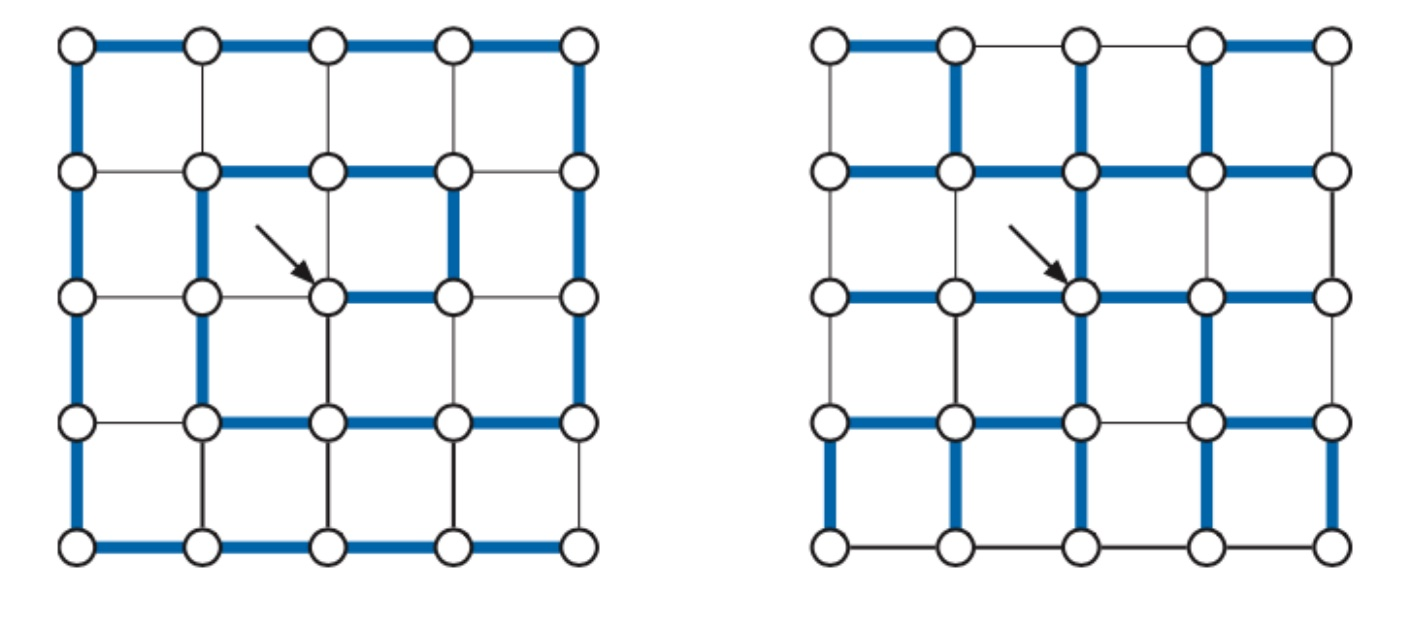
\includegraphics[width=0.8\textwidth]{lecture15/images/spanning-tree.jpg}
\end{itemize}
